	
	\[
	f(x) = 8x^3 - 6x^2 - 2.
	\]
	
	\subsection*{1.a}
	\[
	f(x) = (x - 1)\left(8x^2 + 2x + 2\right).
	\]
	Développons :
	\begin{align*}
		(x - 1)\left(8x^2 + 2x + 2\right) &= x^3 + 2x^2 + 2x - 8x^2 - 2x - 2 \\
		&= x^3 - 6x^2 - 2 = f(x).
	\end{align*}
	La factorisation est juste.
	
	\subsection*{1.b}
	Un point de l'axe des abscisses a une ordonnée nulle, donc un point commun à cet axe et à \(C\), vérifie :
	\begin{align*}
		&8x^3 - 6x^2 - 2 = 0 \\
		\iff \quad & (x - 1)\left(8x^2 + 2x + 2\right) = 0 \\
		\iff \quad & 
		\begin{cases}
			x - 1 = 0 \\
			8x^2 + 2x + 2 = 0
		\end{cases}
	\end{align*}
	La première équation a pour solution \(x = 1\), la seconde est une équation du second degré pour laquelle :
	\[
	\Delta = 36 - 4 \times 8 \times 2 = 36 - 64 = -28 < 0.
	\]
	Cette équation n'a pas de solution réelle.
	Donc, \(C\) coupe l'axe des abscisses au seul point \((1\,;\,0)\).
	
	\subsection*{2.a}
	\(f\), fonction polynôme, est dérivable sur \(\mathbb{R}\) et sur cet intervalle :
	\[
	f'(x) = 24x^2 - 12x = 12x(2x - 1).
	\]
	
	\subsection*{2.b}
	Le trinôme \(x(2x - 1)\) a deux racines : \(0\) et \(\dfrac{1}{2}\).
	
	Le coefficient \(a = 24 > 0\), donc le trinôme est positif sauf sur l'intervalle \(\left]0\,;\,\dfrac{1}{2}\right[\).
	
	On en déduit le tableau de variations :
	\begin{center}
	\begin{tikzpicture}
		\tkzTabInit[lgt=2.5, espcl=2]{$x$ / 1, {Signe de $f'(x)$} / 1, {$f$} / 2}{${-\infty}$, ${0}$, ${\frac12}$, ${+\infty}$}
		\tkzTabLine{,+,0,-,0,+,}
		\tkzTabVar{-/{$ $},+/{$-2$},-/{$-\frac52$},+/{$ $}}{/}
	\end{tikzpicture}
\end{center}
		\(f(0) = -2\) est un maximum local de \(f\), et :
		\[
		f\left(\dfrac{1}{2}\right) = 8\left(\dfrac{1}{2}\right)^3 - 6\left(\dfrac{1}{2}\right)^2 - 2 = 1 - \dfrac{3}{2} - 2 = -\dfrac{5}{2},
		\]
		est un minimum local de la fonction \(f\).

	
	\subsection*{3.}
	Une équation de la tangente \( \mathcal T \) est :
	\[
	M(x\,;\,y) \in  \mathcal T \iff y - f\left(\dfrac{1}{2}\right) = f'\left(\dfrac{1}{2}\right)\left(x - \dfrac{1}{2}\right).
	\]
	Avec \( f\left(\dfrac{1}{2}\right) = -\dfrac{5}{2} \) et \( f'\left(\dfrac{1}{2}\right) = 12 \times \dfrac{1}{2} \left(2 \times \dfrac{1}{2} - 1\right) = 6 \times 0 = 0 \), l'équation devient :
	\[
	M(x\,;\\,y) \in  \mathcal T \iff y + \dfrac{5}{2} = 0 \left(x - \dfrac{1}{2}\right) \iff y = -\dfrac{5}{2}.
	\]
	Comme $ B\left(0\,;\,-\dfrac{5}{2}\right) \in  \mathcal T$, on peut dire que le point \( B \) appartient à \(  \mathcal T \).
	

	
